\documentclass{article}
\usepackage[tmargin=1in,bmargin=1in,lmargin=1.5in,rmargin=1.5in]{geometry}
\usepackage{amsfonts,amsmath,amssymb,amsthm}
\usepackage{mathrsfs}
\usepackage{ccfonts}
\usepackage{relsize,fancyhdr,parskip}
\usepackage{graphicx}

\usepackage{tikz} \usetikzlibrary{shapes, shapes.geometric,
  shapes.symbols, shapes.arrows, shapes.multipart, shapes.callouts,
  shapes.misc,decorations.markings,decorations.shapes}

\pagestyle{fancy}
\lhead{Ben Carriel}
\chead{Math 6510 Problem Set 2}
\rhead{\today}

\parskip 7.2pt
\parindent 8pt

\newcommand{\tab}{\hspace*{2em}}
\newcommand{\tand}{\tab\text{and}\tab}

\DeclareMathOperator{\N}{\mathbb{N}}
\DeclareMathOperator{\Z}{\mathbb{Z}}
\DeclareMathOperator{\Q}{\mathbb{Q}}
\DeclareMathOperator{\R}{\mathbb{R}}
\DeclareMathOperator{\C}{\mathbb{C}}
\DeclareMathOperator{\D}{\mathbb{D}}
\DeclareMathOperator{\T}{\mathbb{T}}
\DeclareMathOperator{\capchi}{\raisebox{2pt}{$\mathlarger{\mathlarger{\chi}}$}}

\DeclareMathOperator{\divides}{\mathrel{|}}
\DeclareMathOperator{\suchthat}{\mathrel{:}}

\DeclareMathOperator{\lra}{\longrightarrow}
\DeclareMathOperator{\into}{\hookrightarrow}
\DeclareMathOperator{\onto}{\twoheadrightarrow}
\DeclareMathOperator{\bijection}{\leftrightarrow}
\DeclareMathOperator{\lap}{\bigtriangleup}

\newcommand{\problem}[1]{\noindent{\textbf{Problem #1}}\\}
\newcommand{\problempart}[1]{\noindent{\textbf{(#1)}}}
\newcommand{\exercise}[1]{\noindent{\textbf{Exercise #1:}}}

\newcommand{\der}[2]{\frac{\partial #1}{\partial #2}}
\newcommand{\norm}[1]{\|#1\|}
\newcommand{\diam}[1]{\text{diam}(#1)}
\newcommand{\seq}[2]{\{#1_{#2}\}_{#2 = 1}^\infty}

\newcommand{\conj}[1]{\overline{#1}}
\newcommand{\cis}[1]{\operatorname{cis}#1}


\newcommand{\real}{\mathrel{\text{Re}}}
\newcommand{\imag}{\mathrel{\text{Im}}}
\newtheorem*{thm}{\\ Theorem}
\newtheorem*{lem}{\\ Lemma}
\newtheorem*{claim}{\\ Claim}
\newtheorem*{defn}{\\ Definition}
\newtheorem*{prop}{\\ Proposition}

\begin{document}
\exercise{1.1.12}

If we are given a homomorphism $f: \pi_1(S^1) \to \pi_1(S^1)$. Because
$\pi_1(S^1)$ is cyclic $f$ is uniquely determined by its value on the
generator $\omega_1$. By definition, $f$ maps loops to loops and
therefore there is some $k$ such that $f([\omega_1]) = [\omega_k]$. I
claim that $f$ induces a homomorphism $\varphi_k: \theta \mapsto
k\theta$ for each $\theta \in S^1$. To see this, note that the loop
$\gamma: \theta \mapsto 2\pi \theta$ satisfies $(\varphi_k \circ
\gamma)(\theta) = 2\pi k\theta$ and so $(\varphi \circ \gamma)(I) =
\omega_k$. We have shown that $(\varphi_k)_*([\omega_1]) =
f_*([\omega_1])$ and so $(\varphi_k)_* = f_*$.

\exercise{1.1.16}

\begin{enumerate}
\item[\textbf{(a)}] Suppose that there were a retraction $r: \R^3 \to
  S^1$. Then there would be some induced homomorphism that there is
  some homomorphism $\pi_1(S^1) \to \pi_1(\R^3)$. Because $r$ is a
  deformation retract this is an injective homomorphism $\Z
  \into 0$, which is impossible.
\item[\textbf{(b)}] Suppose that $r: S^1 \times D^2 \to S^1 \times
  S^1$ were a deformation retraction. If we consider the fundamental
  groups of both spaces
  \begin{align*}
    \pi_1(S^1 \times D^2) \cong \pi_1(S^1) \times \pi_1(D^2) \cong \Z \\
    \pi_1(S_1 \times S_1) \cong \pi_1(S^1) \times \pi_1(S^1) \cong \Z
    \times \Z
  \end{align*}
  Then $r$ induces an injective homomorphism $\Z \times \Z \into
  \Z$. But this is impossible because both each generator $(0,1)$ and
  $(1,0)$ must map to the identity, so the map cannot be injective.
\item[\textbf{(c)}] If there were a retraction $r: S^1 \times D^2 \to
  A$ then there would be some induced homomorphism $\varphi_*:
  \pi_1(A) \to \pi_1(S^1 \times D^2)$. The generator is sent to a loop
  in $X$ that loops around once, and then retraces back on the $S^1$
  factor. This is homotopic to a constant loop. Hence, the induced map
  is trivial, not injective, so we have a contradiction.
\item[\textbf{(d)}] Again, we proceed by contradiction. The space $X =
  D^2 \times D^2$ is clearly path-connected and deformation retracts
  onto a point, hence $\pi_1(X) \cong 0$. Conversely, we know that the
  fundamental group of the figure-eight is $\pi_1(S^1 \vee S^1) \cong
  \Z \ast \Z$. Hence, the deformation retraction $r$ induces an
  injective homomorphism $\Z \ast \Z \into 0$, which is impossible.
\item[\textbf{(e)}] The disk with two points on the boundary
  identified is homotopic to the circle $S^1$, and therefore has
  fundamental group $\Z$. However, the boundary torus has fundamental
  group $\Z \ast \Z$. So if there were a retraction then we would have
  some induced homomorphism $\Z \ast \Z \into \Z$, which should be
  injective. But this is impossible, so there cannot be such a
  retraction.
\item[\textbf{(f)}] To see that the M\"{o}bius strip does not
  deformation retract onto its boundary circle, we suppose that there
  were such a retraction. This retraction would induce a homomorphism
  of the fundamental group, say $\varphi$. Consider the generator for
  the fundamental group of the M\"{o}bius strip and its image under
  $\varphi$. We see that the loop must wrap around twice around the
  circle. So $\varphi: \pi_1(A) \into \pi_1(X)$ is multiplication by
  2. This implies that there is a homomorphism $\Z \onto 2\Z$ that
  restricts to the identity, but this is impossible.
\end{enumerate}

\exercise{1.1.17}

To see the family of non-homotopic retractions $S^1 \vee S^1 \to
S^1$ consider the family
\[
r_n(\theta,\varphi) =
\begin{cases}
  \varphi & \theta = 0 \\
  n\theta & \theta \neq 0
\end{cases}
\]
We need to check the following facts
\begin{enumerate}
\item Each $r_n$ is a deformation rectraction.
\item $r_n \not\simeq r_m$ unless $n = m$.
\end{enumerate}
For (1) we need to verify that the map is continuous and restricts to
the identity on the circle. The latter is clear from the definition
(the identity on the second coordinate). Geometrically, the map is the
identity on the ``left circle'' and loops around the circle $n$ times
on the ``right circle''. The map is continuous on each circle
separately, so we only need check the common point of intersection. We
see that if we set the common point of intersection to $\theta = \phi
= 0$ (reparametrize if not) then the map agrees on the intersection
and is therefore continuous.

To see (2) we note that $r_n$ could not be homotopic to $r_m$ unluss
$m=n$ because otherwise the induced homomorphisms of these maps could
send $[\omega_n] \mapsto [\omega_m]$, which is clearly impossible.

Hence, the family $\{r_n\}_{n\in \Z}$ is an infinite family of
retractions $S^1 \vee S^1 \to S^1$.

\exercise{0.1}

Consider the torus $S^1 \times S^1$ identified with the square
$I\times I$ in the usual way. So
\[
\begin{tikzpicture}[scale=.8]
  % instantiate nodes
  \node (L) at (-3,0) {$S^1 \times S^1 \simeq$};
  \node[draw,circle,inner sep=1pt,fill=none] (TL) at (-1,1) {};
  \node[draw,circle,inner sep=1pt,fill=none] (BL) at (-1,-1) {};
  \node[draw,circle,inner sep=1pt,fill=none] (TR) at (1,1) {};
  \node[draw,circle,inner sep=1pt,fill=none] (BR) at (1,-1) {};
  % draw boundary with orientation
  \draw[->] (TL) -- (0,1);
  \draw (0,1) -- (TR);
  \draw (TR) -- (1,0);
  \draw[->] (BR) -- (1,0);
  \draw[->] (BL) -- (0,-1);
  \draw (0,-1) -- (BR);
  \draw[->] (BL) -- (-1,0);
  \draw (TL) -- (-1,0);
  % generating circles
  \draw[dashed] (0,1) -- (0,-1);
  \draw[dashed] (-1,0) -- (1,0);
\end{tikzpicture}
\]
Consequently, the four corner points of the square are identified as the
same. We will show that the torus with this point removed has the
union of two circles (the dashed lines in the figure above) as a
deformation retract.

Indeed, we can visualize the map as follows: in each quadrant of the
square, draw the line connecting the center of the square to the
corner in that quadrant, and move each point along the line parallel
to this line until you meet one of the inner lines, defining the
two circles.
\[
\begin{tikzpicture}[scale=1.25]
  \node[draw,circle,inner sep=1pt,fill=none] (TL) at (-1,1) {};
  \node[draw,circle,inner sep=1pt,fill=none] (BL) at (-1,-1) {};
  \node[draw,circle,inner sep=1pt,fill=none] (TR) at (1,1) {};
  \node[draw,circle,inner sep=1pt,fill=none] (BR) at (1,-1) {};
  % draw boundary with orientation
  \draw[->] (TL) -- (0,1);
  \draw (0,1) -- (TR);
  \draw (TR) -- (1,0);
  \draw[->] (BR) -- (1,0);
  \draw[->] (BL) -- (0,-1);
  \draw (0,-1) -- (BR);
  \draw[->] (BL) -- (-1,0);
  \draw (TL) -- (-1,0);
  % generating circles
  \draw[dashed] (0,1) -- (0,-1);
  \draw[dashed] (-1,0) -- (1,0);
  % diagonal lines
  \draw[dotted] (TR) -- (0,0);
  \draw[dotted] (TL) -- (0,0);
  \draw[dotted] (BR) -- (0,0);
  \draw[dotted] (BL) -- (0,0);
  % draw x_1 and f(x_1)
  \node (XL) at (-1.2,.5) {\tiny{$x_1$}};
  \node[draw,circle,inner sep=.5pt,fill] (X) at (-1,.5) {};
  \node (FXL) at (-.25,.15) {\tiny{$f(x_1)$}};
  \node[draw,circle,inner sep=.5pt,fill=none] (FX) at (-.5,0) {};
  \draw[->] (X) -- (-.75,.25);
  \draw[] (-.75,.25) -- (FX);
  % same for x_2 and f(x_2)
  \node (YL) at (-1.2,-.5) {\tiny{$x_2$}};
  \node[draw,circle,inner sep=.5pt,fill] (Y) at (-1,-.5) {};
  \node (FYL) at (-.25,-.15) {\tiny{$f(x_2)$}};
  \draw[->] (Y) -- (-.75,-.25);
  \draw[] (-.75,-.25) -- (FX);
  % draw Y_1 and f(Y_1)
  \node (Y1L) at (-.5,1.2) {\tiny{$y_1$}};
  \node[draw,circle,inner sep=.5pt,fill] (Y1) at (-.5,1) {};
  \node (FY) at (-.25,.4) {\tiny{$f(y_1)$}};
  \node[draw,circle,inner sep=.5pt,fill=none] (FY) at (0,.5) {};
  \draw[->] (Y1) -- (-.25,.75);
  \draw[] (-.25,.75) -- (FY);
  % same for Y_2
  \node (Y2L) at (.5,1.2) {\tiny{$y_2$}};
  \node[draw,circle,inner sep=.5pt,fill] (Y2) at (.5,1) {};
  \node (FY) at (.35,.4) {\tiny{$f(y_2)$}};
  \node[draw,circle,inner sep=.5pt,fill=none] (FY) at (0,.5) {};
  \draw[->] (Y2) -- (.25,.75);
  \draw[] (.25,.75) -- (FY);
\end{tikzpicture}
\]
Then we can define the retraction $f$ explicity by defining it
piecewise on each wedge of the square
% solve the stupid linear equations
\[
f(x, y) =
\begin{cases}
  (x + y, 0) & x \leq 0, y \geq 0, |y| \leq |x| \\
  (0, x + y) & x \leq 0, y \geq 0, |y| \geq |x| \\
  (0, y - x) & x \geq 0, y \geq 0, |y| \geq |x| \\
  (x - y, 0) & x \geq 0, y \geq 0, |y| \leq |x| \\
  (y - x, 0) & x \geq 0, y \leq 0, |y| \geq |x| \\
  (0, x + y) & x \geq 0, y \leq 0, |y| \leq |x| \\
  (0, y - x) & x \leq 0, y \leq 0, |y| \leq |x| \\
  (y - x, 0) & x \leq 0, y \leq 0, |y| \geq |x|
\end{cases}
\]
% Prove that $f$ is continuous, check the boundary
To see that $f$ is continuous, we note that it is a straight line on
each of the interiors, so we need only verify continuity on the
boundary. We see that on each of the diagonals, we follow a straight
line to the center of the square, so we agree. Finally, we see that if
either $x,y = 0$ then the map is the identity (as it should be because
it is a retraction. Hence, $f$ is continuous.

 \exercise{0.3}
\begin{enumerate}
\item[\textbf{(a)}] Let $f: X \to Y$ and $g: Y \to Z$ be homotopy
  equivalences. This guarantees the existence of maps $f': Y \to X$
  and $g': Z \to Y$ such that $ff' = f'f = 1$ and $gg' = g'g =
  1$. So
  \[
  (g \circ f)(f' \circ g') = g \circ (f' \circ f) \circ g = g \circ g' = 1
  \]
  Similarly,
  \[
  (f'\circ g')(g \circ f) = f' \circ (g' \circ g) \circ f = f' \circ f = 1
  \]
  So, $f\circ g$ is a homotopy equivalence as well.

  This establishes that homotopy equivalence is an equivalence
  relation because we have relfexivity (use the identity map),
  symmetry (because $fg = gf = 1$), and the above established
  transitivity.
\item[\textbf{(c)}] Now suppose that $h$ is homotopic to a homotopy
  equivalence $f$. Because $f$ is a homotopy equivalence we have a map
  $g$ such that $fg = gf = 1$.
\end{enumerate}

\exercise{0.4}

Suppose that $X$ deformation retracts to $A$ in the weak sense and
consider the inclusion map $i: A \into X$. We must have some homotopy
$H(t,s)$ such that $H_0 = 1$, $H_1(X) \subset A$ and $H_t(A) \subset
A$ for each $t$. We will see that $H_1$ is a two-sided inverse for
$i$. So we need to show first that $H_1 \circ i = 1$. Consider the
homotopy given by $F_t = H_{1-t}|_A$. So that $F_0 = H_1 \circ i$ and
$F_1 = H_0 \circ i = 1$. Now we need to see that $i \circ H_1 = 1$. We
then consider the homotopy $F_t = H_{1-t}$. We see that $H_1 = i \circ
H_1$ because $H_1(X) \subset A$. Moreover, $H_0 = 1$ so we are done.

\exercise{0.5}

Suppose that $X$ deformation retracts onto a point $x \in X$. Let
$H(t,s)$ be a homotopy for this retraction. Let $U$ be a neighborhood
of $x$ and consider its set of preimages under $H$
\[
H^{-1}(U) = \{(t,x) \suchthat H_t(x) \in U\}
\]
Now observe that $I \times \{x\} \subset U$ by the definition of a
retraction. For each $t$ we construct a neighborhood $U_t$ containing
$x$ and a neighborhood $I_t$ of $t$ such that $U_t \times J_t \subset
H^{-1}(U)$ because $H^{-1}(U)$ is open. Then we note that
\[
I \times \{x\} \subset \bigcup_{t \in I} U_t \times I_t
\]
Because $I \times \{x\}$ is compact, we can find a finite subcover
such that
\[
I \times \{x\} \subset \bigcup_{k=1}^n U_{t_k} \times I_{t_k}
\]
We can then extract our deired neighborhood $V$ by setting
\[
V = \bigcap_{k=1}^n U_{t_k}
\]
So $V$ is an open neighborhood of $x$ and $H_t(V) \subset U$ for each
$t$.

If we then look at the inclusion map $i: V \into U$ then we see that
the map $H_t \circ i$ gives a homotopy $G(t,s)$ between $H_0 = i$ and
$H_1$, the constant map to $x$. So $i$ is nullhomotopic.

\exercise{0.6}
\begin{enumerate}
\item[\textbf{(a)}] To see that $X$ deformation retracts onto $\{x_0\}
  \times \{0\}$, we construct the retraction. We begin by retracting
  each interval $\{r\} \times [0,1-r]$ to $\{r\} \times \{0\}$ via the
  straight-line retraction. We then compose this with the retraction
  of $\{0\} \times [0,1]$ onto the point $\{0\}$. Finally, because the
  interval is contractible, we retract onto the desired point $\{x_0\}
  \times \{0\}$ (see Exercise 0.5).

  The difficulty is seeing why a similar construction does not hold
  elsewhere in $X$. To see the difference, consider some other point
  $x = \{r\} \times \{h\}$ in $X$. If there were some deformation
  retract $f_t$ then $f_t$ must be homotopic to a constant map on some
  neighborhood $U$ of $x$. Since $X$ is path-connected, but
  $X\setminus ([0,1] \times \{0\})$ is not, we see that $f_t$ must
  restrict to the identity on $[0,1] \times \{0\}$, unless it
  contracts to a point on $[0,1] \times \{0\}$. But this contradicts
  the fact that $f_t$ restricts to the identity on $V \subset U$.
\item[\textbf{(b)}] We first observe that $Y$ is contractible. To see
  this use the straight line homotopy on each copy of the $X_i$ to
  project onto the bold line (see figure on pg. 18). This line is
  homotopy equivalent to $\R$ and therefore is contractible. Hence, we
  can send the identity to a constant map by composing the projection
  maps with the contraction of the center line. This shows that $Y$
  is contractible.

  Now we need to show that $Y$ does not deformation retract onto any
point. Suppose that there were such a point $y \in Y$ such that $Y$
deformation retracts onto $y$. Then any open neighborhood $U$ of $y$
would have to contain a neighborhood $V$ of $y$ such that the
inclusion map $V \into U$ is nullhomotopic (see Exercise
0.5). However, this is impossible because any $V$ must intersect
non-path connected parts of $U$ (due to density).
\item[\textbf{(c)}] To see that there is a deformation in the weak
sense of $Y$ onto $Z$ we construct it piecewise by looking at the
``union'' of the retractions on the individual copies of $X$. More
precisely, we note that $Y = \bigcup_{n\in \Z} X_i$ where each $X_i$
is a copy of $X$ and so we consider the homotopy $f_t^{(i)}$ as
described in \textbf{(a)}. We then define the deformation retraction
piecewise on each copy of $X$. Because these agree on the boundary of
each of the $X_i$ we see that this is a valid retraction in the weak
sense.

  However, $Z$ is homeomorphic to $\R$. Consequently, we see that $\Z$
must retract onto a point, necause $\R$ retracts onto a point. Hence,
if there were a true retraction $Y \to Z$, then it would imply that
$Y$ deformation retracts onto a point, but we showed in \textbf{(b)}
that this is impossible. As a result, there is no true deformation
retraction.
\end{enumerate}

\exercise{0.9}

Suppose that $X$ is a contractible space and that $A$ is a retract of
$X$. Let $f$ be the retraction $X \onto A$ and suppose that $H(t,s)$
is a homotopy connecting the identity on $X$ to the constant map. If
we compose with the canonical inclusion map $i: A \into X$ then we get
a homotopy
\[ H': A \times I \to X \times I \to X \to A
\] This is a homotopy between the identity on $A$ and the constant
map.

\exercise{0.10}

We need to prove the following
\begin{enumerate}
\item A space $X$ is contractible iff every map $f: X \to Y$ for
arbitrary $Y$, is nullhomotopic.
\item $X$ is contractible iff every map $f: Y \to X$ is nullhomotopic.
\end{enumerate} For (1) we suppose that $X$ is contractible. Then we
can find some point $x \in X$ and homotopy $H: X \times I \to X$ such
that $H_0 = 1$ and $H_1 = x$. Then the composition with $f: X \to Y$
gives $f \circ H: X \times Y \to Y$, which is a homotopy from $f$ to
the constant map at $f(x)$. So $f$ is nullhomotopic. Conversely,
suppose that every map $f: X \to Y$ for all $Y$ is nullhomotopic. Then
in particular, if we set $Y = X$ and $f = 1$ then the identity is
nullhomotopic and $X$ is contractible.

For (2) we again begin with $X$ contractible. If we look at the map
$f: Y \to X$, then the map $F: Y \to I \to X$ given by $(y,t) \mapsto
H(f(y),t)$ is a homotopy from $f$ to the constant map at $a$. So $f$
is nullhomotopic. In the reverse direction, we suppose that every map
$f: Y \to X$ is nullhomotopic. Then we have that the identity map $X
\to X$ is nullhomotopic. Thus, $X$ is contractible.

\exercise{A1}

Consider the closed orientable surface of genus 2, $\T_2$. We label
the four generators for $\pi_1(\T_2)$ as follows,
\[
\begin{tikzpicture}[scale=.75] % lines comprising the torus \draw
(-2.2,0) to[bend left] (-.7,0); \draw (-2.3,.1) to[bend
right](-.6,.1); \draw (.7,0) to[bend left] (2.2,0); \draw (.6,.1)
to[bend right] (2.3,.1); \draw[rotate=0] (0,0) ellipse (100pt and
50pt); % center dot, and generating loops \coordinate (Center) at
(0,-1); \node[draw,circle,inner sep=1pt,fill] at (0,-1) {}; \draw
(Center) .. controls (-.5,3) and (-6,-1) .. (Center); \draw (Center)
.. controls (.5,3) and (6,-1) .. (Center); \draw[dashed] (Center)
to[bend left] (-1.4,-.15); \draw (-1.4,-.15) to[bend left] (Center);
\draw (Center) to[bend left] (1.4,-.15); \draw[dashed] (1.4,-.15)
to[bend left] (Center); % Labels for the paths \node at (-1.5,1)
{$a$}; \node at (-1.3,-.65) {$b$}; \node at (1.5,1) {$c$}; \node at
(1.3,-.65) {$d$};
\end{tikzpicture}
\] We can identify the above figure with the following,
\[
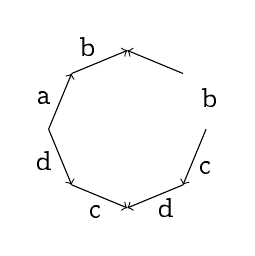
\begin{tikzpicture}[decoration=triangles] % label sides \node at
(.5,1) {a}; \node at (1.05,.4) {b}; \node at (-.5,1.05) {b}; \node at
(-1.05,.4) {a}; \node at (.5,-1) {d}; \node at (1,-.5) {c}; \node at
(-.4,-1.05) {c}; \node at (-1.05,-.4) {d}; % create path nodes \path
(0,0) coordinate (origin); \path (0:1cm) coordinate (P0); \path
(1*45:1cm) coordinate (P1); \path (2*45:1cm) coordinate (P2); \path
(3*45:1cm) coordinate (P3); \path (4*45:1cm) coordinate (P4); \path
(5*45:1cm) coordinate (P5); \path (6*45:1cm) coordinate (P6); \path
(7*45:1cm) coordinate (P7); % Draw the edges of the pentagon \draw[->]
(P0) -- (P1); \draw[->] (P1) -- (P2); \draw[<-] (P2) -- (P3);
\draw[<-] (P3) -- (P4); \draw[->] (P4) -- (P5); \draw[->] (P5) --
(P6); \draw[<-] (P6) -- (P7); \draw[<-] (P7) -- (P0);
\end{tikzpicture}
\] If we look at the fundamental group of an individual torus,
$\pi_1(\T) = \Z \times \Z$, we see that if we map each generator of
$\pi_1(T)$ to a set of loops, $a,b$ and $c,d$, respectively. Then we
can generate the fundamental group of $\T_2$ by joining all of these
at a point. To get the homomorphism onto the free abelian group of
rank four we notice that the path around the boundary is given by
$aba^{-1}b^{-1}cdc^{-1}d^{-1}$, which is an element of the free
product of the groups generated by each loop. When written in group
notation this is the product of the commutators $[a,b]\cdot[c,d]$. If
$C$ is the commutator subgroup of $\pi_1(\T_2)$ then $\pi_1(G)/C$ is
the abelianization of the free product $\Z \ast \Z \ast \Z \ast \Z$,
or the free abelian group of rank 4. The homomorphism is given
explicitly by $x \mapsto xC$.
\end{document}